% *********************************************************************
% © 2010–2022 Jeremy Sylvestre
%
% Permission is granted to copy, distribute and/or modify this document
% under the terms of the GNU Free Documentation License, Version 1.3 or
% any later version published by the Free Software Foundation; with no
% Invariant Sections, no Front-Cover Texts, and no Back-Cover Texts. A
% copy of the license is included in the appendix entitled “GNU Free
% Documentation License” that appears in the output document of this
% PreTeXt source code. All trademarks™ are the registered® marks of
% their respective owners.
%
% *********************************************************************

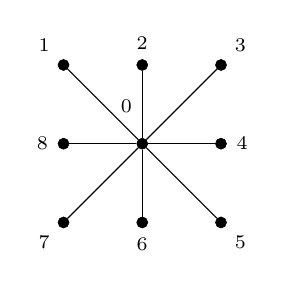
\begin{tikzpicture}[
	vertex/.style={ circle, draw, very thin, fill, inner sep=0pt, minimum size=4pt },
	vertexg/.style={ black!40!white, circle, draw, very thin, fill, inner sep=0pt, minimum size=4pt },
	vertexo/.style={ circle, draw, very thin, inner sep=0pt, minimum size=4pt }
]

\node at (0,0) (zero) [vertex,label={[xshift=-0.2cm, yshift=0.2cm]$\scriptstyle 0$}] {};
\node at (-1,1) (one) [vertex,label=above left:$\scriptstyle 1$] {};
\node at (0,1) (two) [vertex,label=above:$\scriptstyle 2$] {};
\node at (1,1) (three) [vertex,label=above right:$\scriptstyle 3$] {};
\node at (1,0) (four) [vertex,label=right:$\scriptstyle 4$] {};
\node at (1,-1) (five) [vertex,label=below right:$\scriptstyle 5$] {};
\node at (0,-1) (six) [vertex,label=below:$\scriptstyle 6$] {};
\node at (-1,-1) (seven) [vertex,label=below left:$\scriptstyle 7$] {};
\node at (-1,0) (eight) [vertex,label=left:$\scriptstyle 8$] {};
\foreach \p in {one,two,three,four,five,six,seven,eight}
  \draw (zero) to (\p);

\end{tikzpicture}
